\section{Hybrid Parallel Performance}

Runtime performance is investigated through the hybrid parallel implementation of a simple ``mini-application.''
%
This mini-application generates a parallel distributed sparse matrix and then applies conjugate gradient solution algorithm iterations to that system of equations.
%
The sparse matrix is generated from applying a 27-point stencil to a regular three dimensional grid, resulting in 27 non-zero coefficients per matrix row associated with locations in the interior of the grid.
%
The distribution of the sparse matrix is obtained by applying a recursive coordinate bisection \cite{RCB:1989} partitioning to the grid.


Performance is studied by running this mini-application on a hybrid parallel machine.
%
This mini-application is run in the following three modes.
\begin{blist}
\item An all-MPI mode where one MPI process is run on each CPU core.
\item A one-MPI-process-per-node mode where one worker thread is created for each additional CPU core on the node.
\item A one-MPI-process-per-socket mode where one MPI process is run on each CPU socket and one worker thread is created for each additional CPU core on the socket.
\end{blist}


\clearpage
\subsection{Parallel Conjugate Gradient Algorithm Iteration}

A simple conjugate gradient solver algorithm for a sparse linear system of equations is implemented using two-level parallelism: MPI for inter-process parallelism and ThreadPool for intra-process parallelism.
%
This parallel algorithm can be implemented with a small number of basic linear algebra subprogram (BLAS) kernels:
$\mathbf{y}=\mathbf{x}$,
$dot(\mathbf{x},\mathbf{y})$,
$\mathbf{y}=\alpha*\mathbf{x}+\beta*\mathbf{y}$, and
$\mathbf{y}=\mathbf{A}*\mathbf{x}$.
%
For intra-process thread-level parallelism each call to a kernel will have runtime overhead starting and waiting on the local threads.
%
This overhead can be minimized by \emph{fusing} parallel kernels, as presented in Algorithm~\ref{alg:CG-fused}.


\begin{algorithm}[h]
\SetKwInOut{KwInOut}{InOut}
\SetAlgoLined
\DontPrintSemicolon
\Begin(parallel symmetric conjugate gradient algorithm){
\KwIn{$\mathbf{A} \equiv$ sparse symmetric matrix}
\KwIn{$\mathbf{b} \equiv$ right-hand-side vector}
\KwInOut{$\mathbf{x} \equiv$ initial guess, solution vector}
\KwData{$\mathbf{r} \equiv$ residual vector}
\KwData{$\mathbf{p} \equiv$ solution vector update, length = \# columns of $\mathbf{A}$}
\KwData{$\mathbf{Ap} \equiv$ residual vector update}
$\mathbf{r} = \mathbf{b}$ \tcc*{parallel} \;
$\mathbf{p} = \mathbf{x}$ \tcc*{parallel} \;
$\mathbf{Ap} = \mathbf{A} * \mathbf{p}$ \tcc*{parallel} \;
$\mathbf{r} = \mathbf{r} - \mathbf{Ap}$ ; $\delta = dot(\mathbf{r},\mathbf{r})$ \tcc*{fused parallel} \;
$\beta = 0 $ \tcc*{serial} \;
\While(\tcc*[f]{serial}){$\mathit{tolerance} < \delta$ and within iteration limit }{
  $\mathbf{p} = \mathbf{r} + \beta * \mathbf{p}$ \tcc*{parallel} \;
  $\mathbf{Ap} = \mathbf{A} * \mathbf{p}$ ; $\gamma = dot(\mathbf{Ap},\mathbf{p}) $ \tcc*{fused parallel} \;
  $\alpha = \delta / \gamma $ ; $\beta = \delta $ \tcc*{serial} \;
  $\mathbf{x} = \mathbf{x} + \alpha * \mathbf{p}$ ; $\mathbf{r} = \mathbf{r}- \alpha * \mathbf{Ap}$ ; $\delta = dot(\mathbf{r},\mathbf{r})$ \tcc*{fused parallel} \;
  $\beta = \delta / \beta$ \tcc*{serial} \;
}
}
\caption{Conjugate gradient algorithm with \emph{fused} parallel kernels}
\label{alg:CG-fused}
\end{algorithm}


In the conjugate gradient algorithm the matrix vector multiplication step is immediately followed by an inner product of the input and output vectors.
%
Fusing these steps into a single parallel kernel eliminates the thread-wait and thread-start overhead associated with completing the first kernel and starting the second kernel.
%
A thread-parallel work kernel for this operation could separate or fuse these steps.


\clearpage

\subsection{Hybrid Fused Parallel Sparse Matrix Vector Multiplication}

Algorithm~\ref{alg:FusedMXV} describes a hybrid parallel fused implementation of the matrix-vector multiply followed by a dot product of the input and output vectors.
%
In this algorithm the thread work kernel performs both the matrix-vector multiply and the dot product.
%
Internal to the thread work kernel, these two operations can be implemented separate serial linear algebra kernels.


\begin{algorithm}[h]
\SetKwInOut{KwInOut}{InOut}
\SetKwBlock{Call}{Call}{end}
\SetKwBlock{CallThread}{Each thread calls}{end}
\SetKwInOut{KwInOut}{InOut}
\SetAlgoLined
\DontPrintSemicolon
\Begin( Fused parallel function: \mbox{$\gamma = dot( ( \mathbf{y} = \mathbf{A} * \mathbf{x} ) , \mathbf{x} )$}){
\KwIn{$\mathbf{A}_\mathrm{P} \equiv$ this process' rows of matrix $\mathbf{A}$}
\KwInOut{$\mathbf{x}_\mathrm{P} \equiv$ this process' portion of vector $\mathbf{x}$ spans columns of $\mathbf{A}_\mathrm{P}$}
\KwOut{$\mathbf{y}_\mathrm{P} \equiv$ this process' portion of vector $\mathbf{y}$}
\KwOut{$\gamma \equiv$ result of dot product on all processes}
\BlankLine
Gather off-process columns into $\mathbf{x}_\mathrm{P}$ via MPI communication \;
\BlankLine
\Call( \textnormal{TPI\_Run\_threads\_reduce( work\_kernel , reduction\_kernel )}){
\BlankLine
\CallThread( \textnormal{work\_kernel} ){
\KwIn{$\mathbf{A}_\mathrm{P,T} \equiv$ this thread's span of matrix $\mathbf{A}_\mathrm{P}$}
\KwIn{$\mathbf{x}_\mathrm{P} \equiv$ this process' complete input vector}
\KwOut{$\mathbf{y}_\mathrm{P,T} \equiv$ this thread's span of vector $\mathbf{y}_\mathrm{P}$}
\KwOut{$\gamma_\mathrm{T} \equiv$ this thread's contribution to $\gamma$}
\BlankLine
$\mathbf{y}_\mathrm{P,T} = \mathbf{A}_\mathrm{P,T} * \mathbf{x}_\mathrm{P}$ \;
$\gamma_\mathrm{T} = dot( \mathbf{y}_\mathrm{P,T} , \mathbf{x}_\mathrm{P,T} )$ \;
}
\CallThread( \textnormal{reduction\_kernel} ){
\KwInOut{$\gamma_\mathrm{T} \equiv$ this thread's contribution to $\gamma$}
\KwIn{$\gamma_\mathrm{U} \equiv$ another thread's contribution to $\gamma$}
\BlankLine
$\gamma_\mathrm{T} = \gamma_\mathrm{T} + \gamma_\mathrm{U}$ \;
}
}
Reduce $\gamma$ among all processes  via MPI\_Allreduce
}
\caption{Fused hybrid parallel kernel for \mbox{$\gamma = dot( ( \mathbf{y} = \mathbf{A} * \mathbf{x} ) , \mathbf{x} )$} }
\label{alg:FusedMXV}
\end{algorithm}

\clearpage

\subsection{Performance Study}

This performance study was run on an HPC cluster at Sandia National Laboratories.
%
This cluster (called \emph{glory}) consists of 272 quad-socket compute nodes with 2.2 GHz AMD quad-core CPUs, and an Infiniband interconnect.
%
The mini-application was compiled at optimization level 3, using the Intel-11 compiler, OpenMPI, and standard pthreads.


The mini-application is run on 4, 8, 16, and 32 compute nodes with
\begin{blist}
\item one MPI process on each available core,
\item one MPI process on each available socket and worker threads created on each remaining core, and
\item one MPI process on each node and worker threads created on each remaining core.
\end{blist}
%
The compute node architecture provides non-uniform memory access (NUMA) performance between the CPUs and main memory.
%
As such the Linux non-uniform memory access control (numactl) capability is used to attach MPI processes to sockets or cores.



\subsubsection{Processes versus Threads}

Results from the performance studies are summarized in Figures~\ref{fig:CGPerf:np4}-\ref{fig:CGPerf:np32}.
%
Each of these graphs is for a fixed number of compute nodes and thread, where each line is for one of the three approaches to allocating MPI process and pthreads to cores (MPI-per-core, MPI-per-socket,and MPI-per-node).
%
The objective of these studies is to compare the performance of the three MPI process versus pthread allocation approaches over a range of problem sizes.
%
This comparison method is chosen to make apparent the impact of cache memory and non-uniform memory access on performance.


Each graph (Figures~\ref{fig:CGPerf:np4}-\ref{fig:CGPerf:np32}) plots the aggregate gigaflop performance attained from parallel CG iterations over a range of problem size, from less than 1e4 to more than 1e7 grid points (matrix rows).
%
For small problem sizes of less than 1e4 grid points the message passing, thread startup, and thread completion overhead dominates performance --- yielding poor gigaflop performance.
%
From this small problem size, performance of the hybrid parallel approaches improves rapidly with problem size.
%
However, once the matrix and vectors exceeds the CPUs' cache size performance drops significantly and becomes limited by main memory access performance.
%
Furthermore, the performance drop of the MPI-per-node approach is worse due to threads running on four different sockets accessing shared memory allocated physically near its own socket.
%
This is in contrast to the MPI-per-socket and MPI-per-core results where each thread only accesses NUMA memory associated with its own socket.

\clearpage

The approach of using one-MPI-process-per-socket, with one thread per core, consistently yielded the best performance.
%
This result is especially pronounced for the strong scaling (\emph{i.e.}, speed up) results presented in Figures~\ref{fig:CGPerf:scaling1M}~and~\ref{fig:CGPerf:scaling1.7M}.
%
These results are for matrices with 1M and 1.7M rows respectively.

Strong scaling results presented in Figures~\ref{fig:CGPerf:scaling1M}~and~\ref{fig:CGPerf:scaling1.7M} are problem dependent.
%
This dependency is readily apparent in Figure~\ref{fig:CGPerf:scaling} which plots performance versus problem size for each of the one-MPI-process-per-socket test cases.


The following three observations are apparent from these performance results.
\begin{blist}
\item Strong scaling of the one-MPI-process-per-node and one-MPI-process per socket is dramatically better than the one-MPI-process-per-core for small matrices.
\item Performance of the one-MPI-process-per-node mode is significantly worse for large matrices.
\item Performance of the one-MPI-process-per-socket mode is better for (nearly) all sizes of matrices.
\end{blist}
%
Thus for this mini-application running on Sandia's glory cluster, with its NUMA compute nodes, the best performance is achieved with a hybrid parallel strategy of allocating one MPI process to each CPU socket and then applying thread parallelism to utilize the three remaining cores within each socket.
%
The degree to which performance is better depends upon the size and layout of the computational data relative to the CPU cache.
%
If this data can be held in CPU cache for a relatively large number of computations then performance is show to be dramatically better.



\begin{figure}[h]
\center
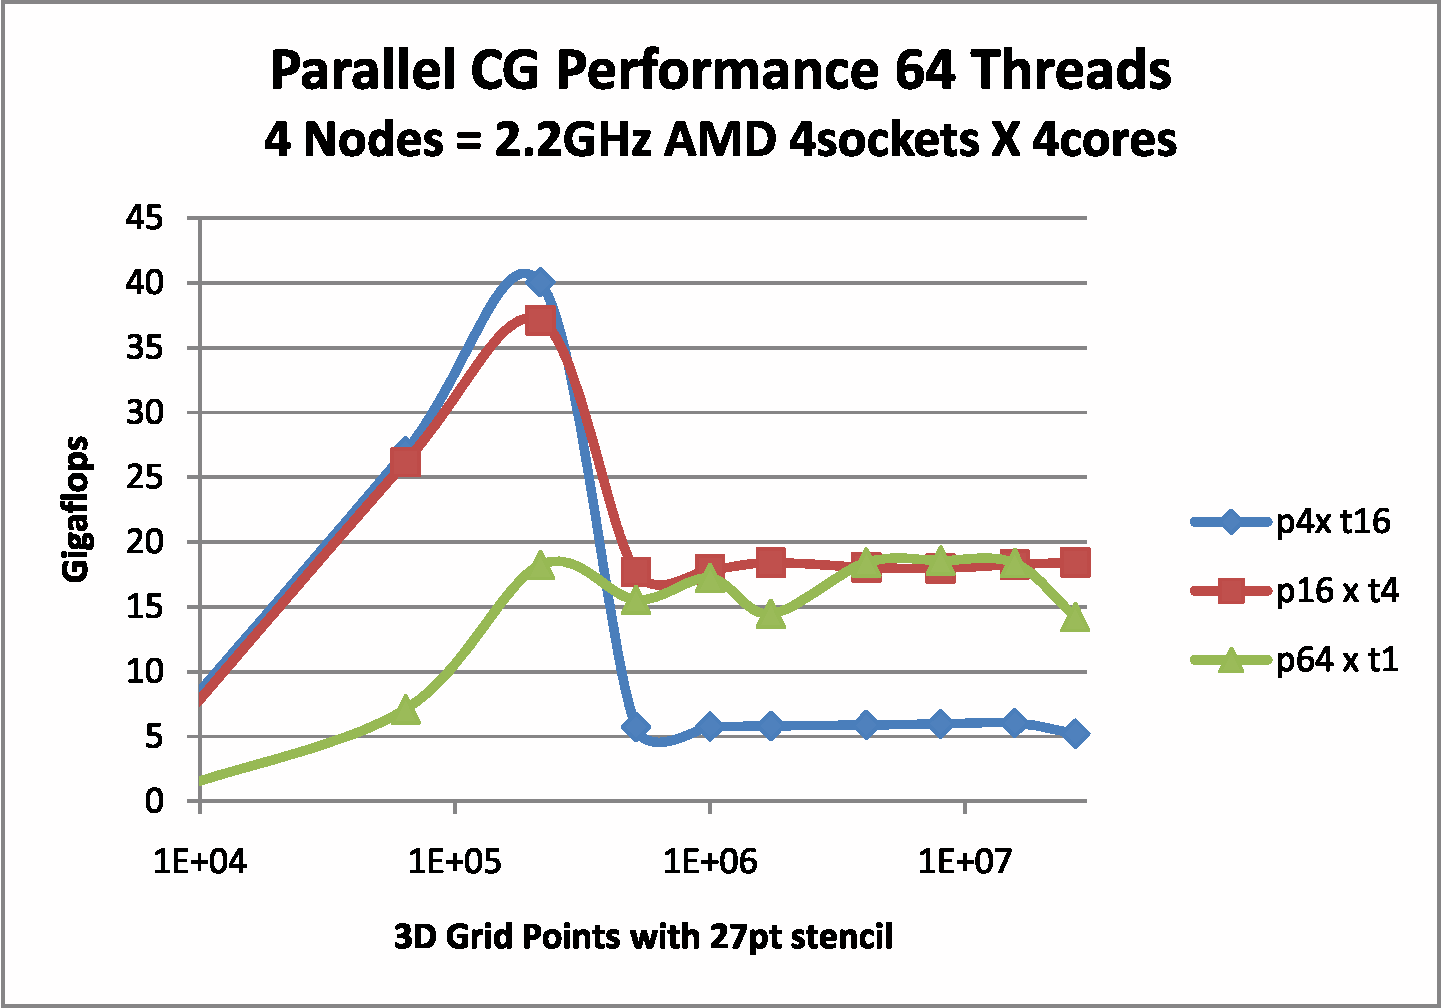
\includegraphics[viewport=1in 0.5in 8.5in 6.5in,angle=0,scale=0.5]{figures/test-hhpccg-intel-11-1-mpi-exe-np4-no-overlap-2}
\caption{Comparison of hybrid parallel conjugate gradient iteration performance for 4 compute nodes with 64 threads: p4 x t16 = one MPI process per node, p16 x t4 = one MPI process per socket, and p64 x t1 = one MPI process per core.}
\label{fig:CGPerf:np4}
\end{figure}

\begin{figure}[h]
\center
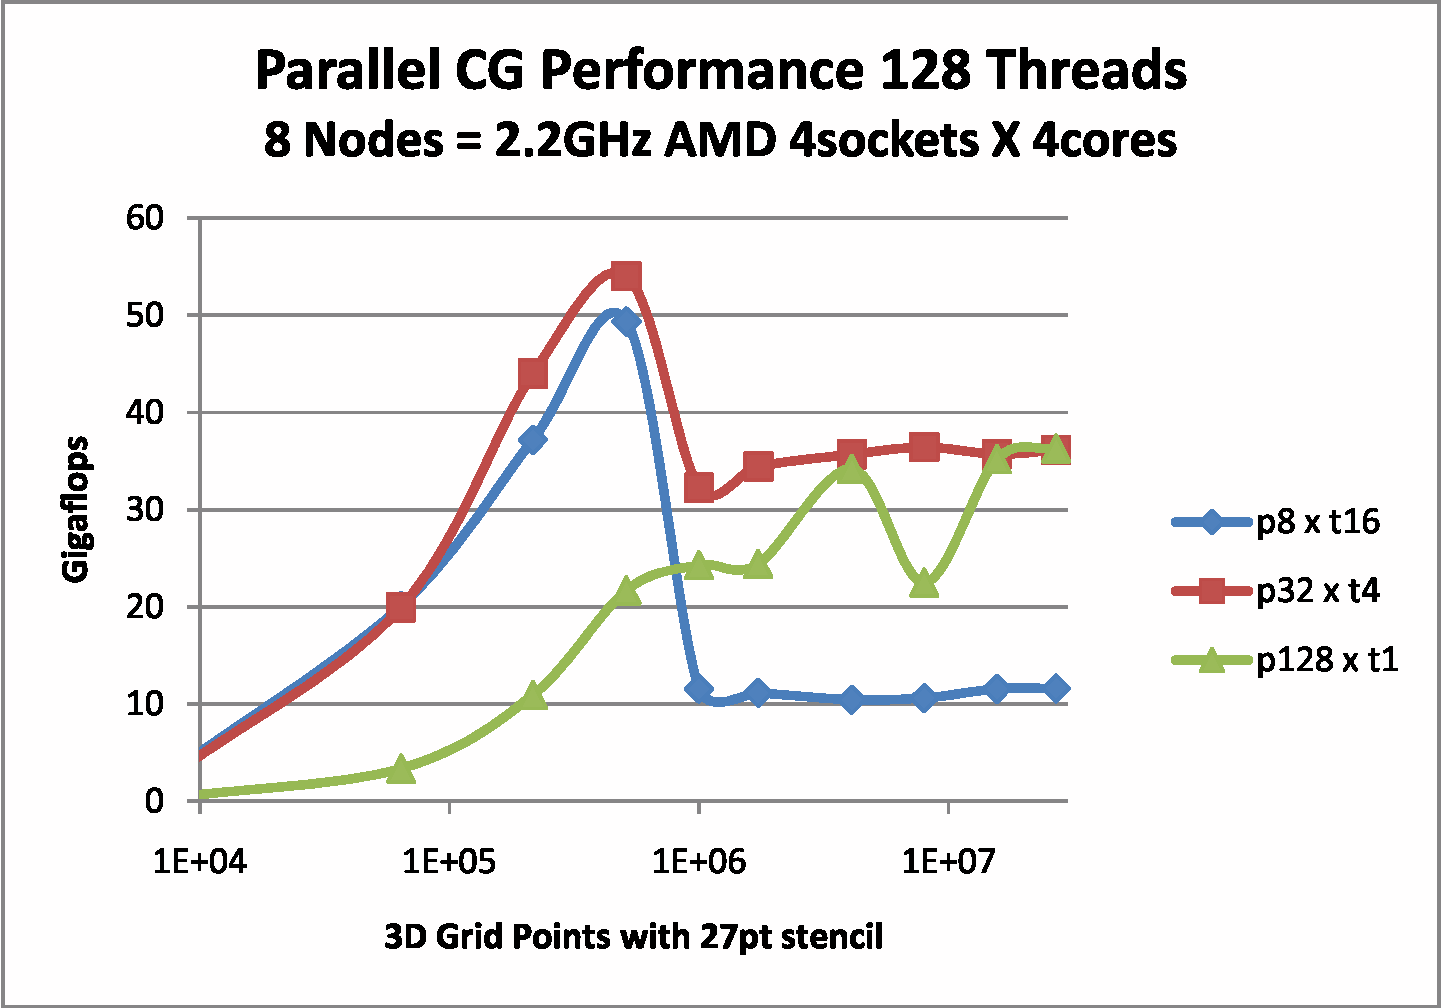
\includegraphics[viewport=1in 0.5in 8.5in 6.5in,angle=0,scale=0.5]{figures/test-hhpccg-intel-11-1-mpi-exe-np8-no-overlap-2}
\caption{Comparison of hybrid parallel conjugate gradient iteration performance for 8 compute nodes with 128 threads: p8 x t16 = one MPI process per node, p32 x t4 = one MPI process per socket, and p128 x t1 = one MPI process per core.}
\label{fig:CGPerf:np8}
\end{figure}

\begin{figure}[h]
\center
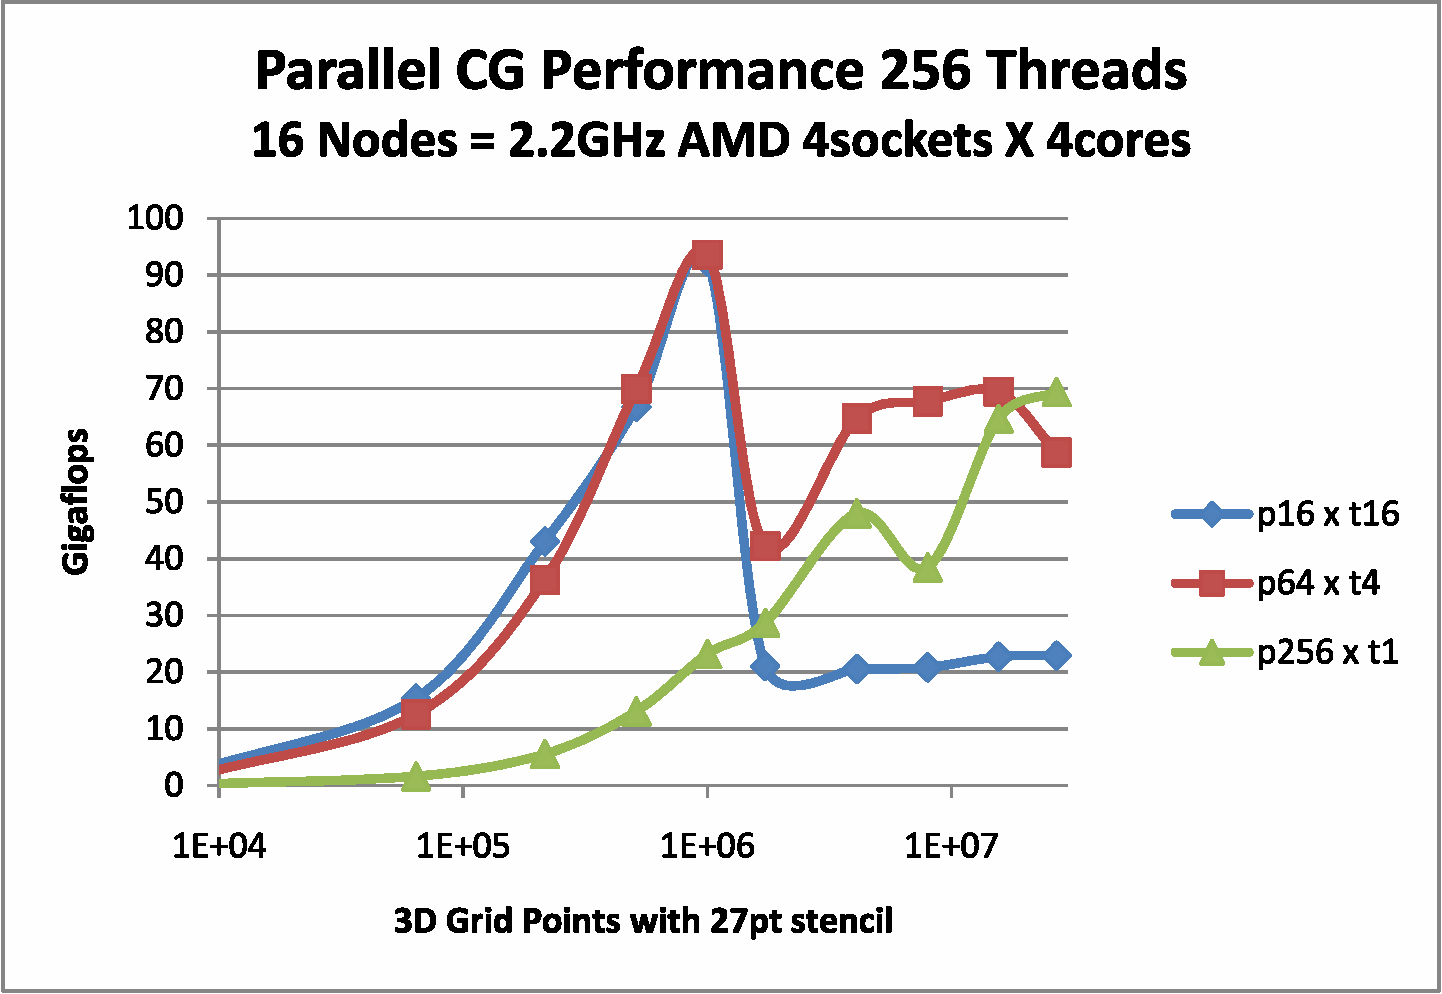
\includegraphics[viewport=1in 0.5in 8.5in 6.5in,angle=0,scale=0.5]{figures/test-hhpccg-intel-11-1-mpi-exe-np16-no-overlap-2}
\caption{Comparison of hybrid parallel conjugate gradient iteration performance for 16 compute nodes with 256 threads: p16 x t16 = one MPI process per node, p64 x t4 = one MPI process per socket, and p256 x t1 = one MPI process per core.}
\label{fig:CGPerf:np16}
\end{figure}

\begin{figure}[h]
\center
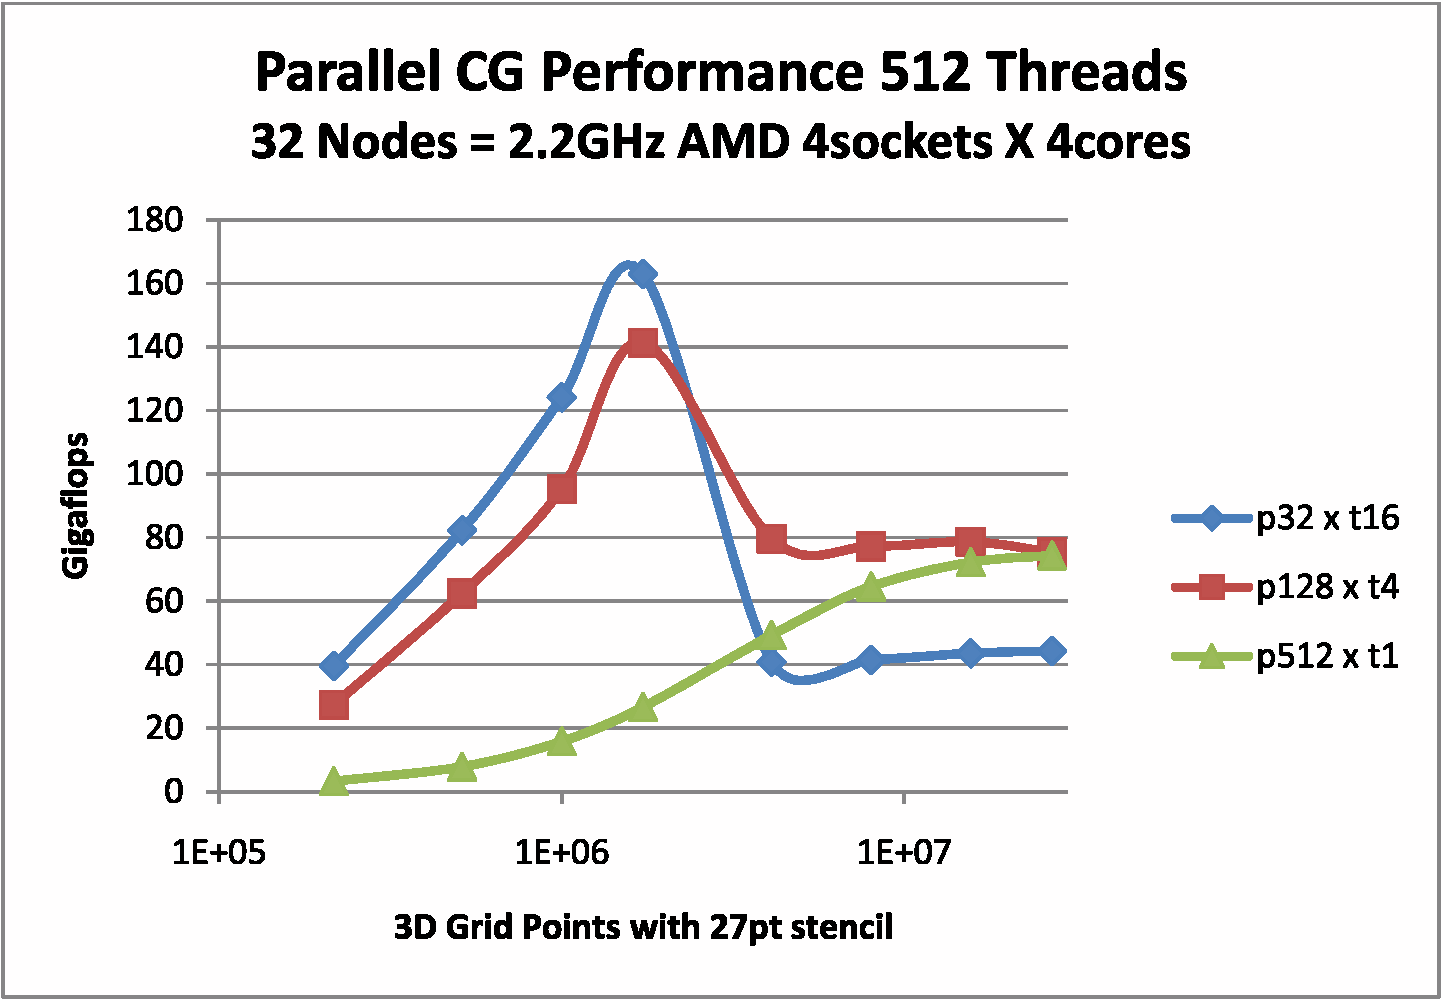
\includegraphics[viewport=1in 0.5in 8.5in 6.5in,angle=0,scale=0.5]{figures/test-hhpccg-intel-11-1-mpi-exe-np32-no-overlap}
\caption{Comparison of hybrid parallel conjugate gradient iteration performance for 32 compute nodes with 512 threads: p32 x t16 = one MPI process per node, p128 x t4 = one MPI process per socket, and p512 x t1 = one MPI process per core.}
\label{fig:CGPerf:np32}
\end{figure}


\begin{figure}[h]
\center
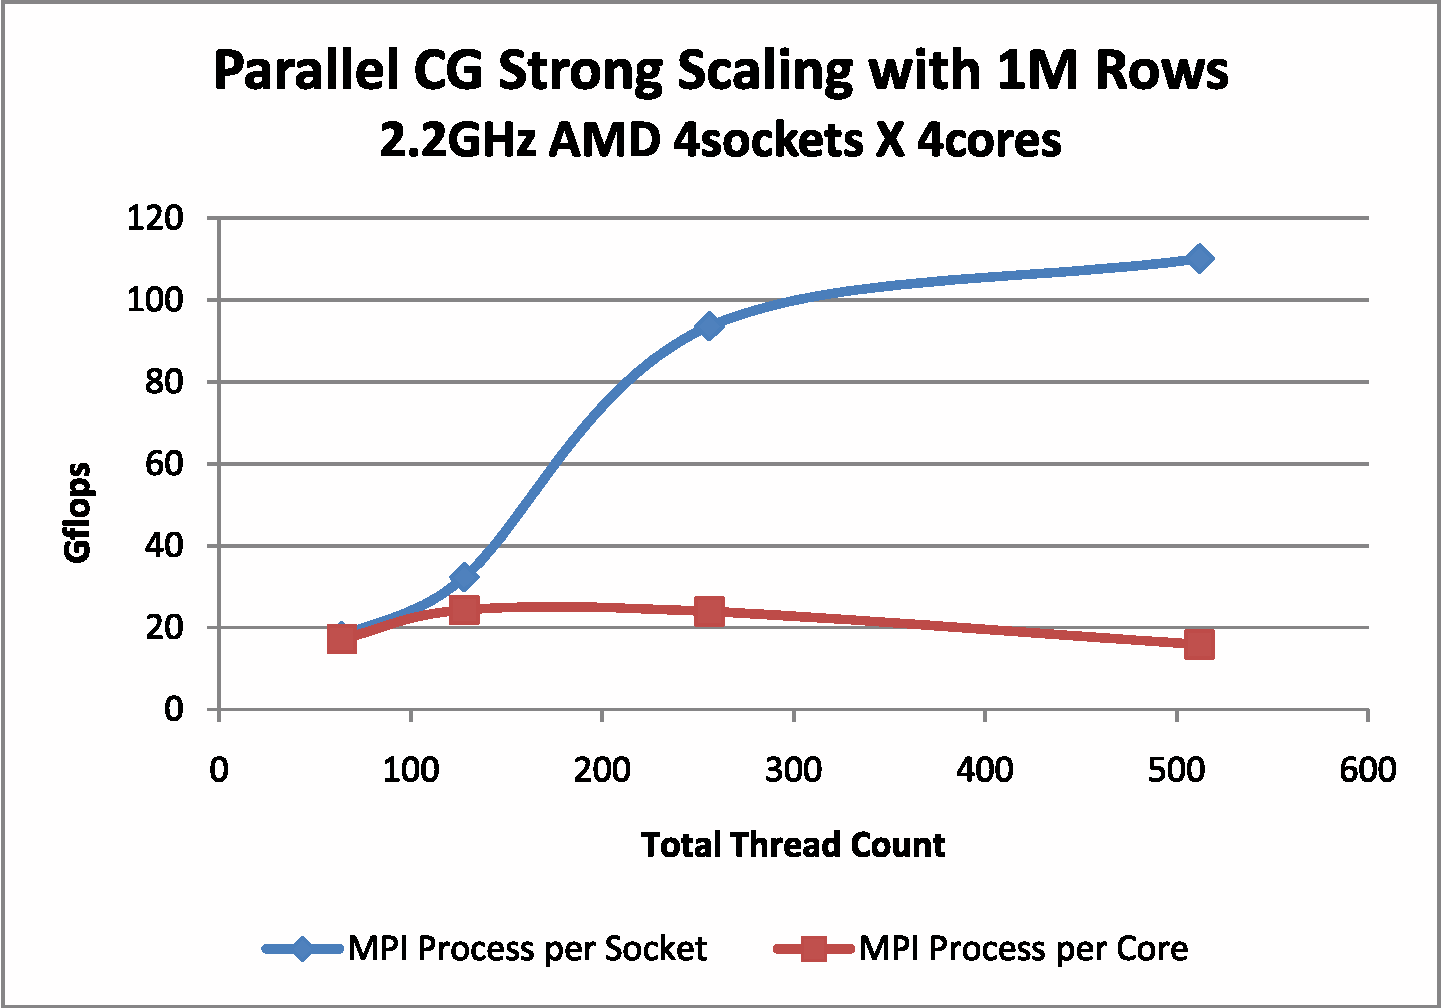
\includegraphics[viewport=1in 0.5in 8.5in 6.5in,angle=0,scale=0.5]{figures/StrongScaling1000k}
\caption{Hybrid parallel conjugate gradient iteration strong scaling for 1M rows: one MPI process with 4 threads per CPU socket versus one MPI process per CPU core.}
\label{fig:CGPerf:scaling1M}
\end{figure}

\begin{figure}[h]
\center
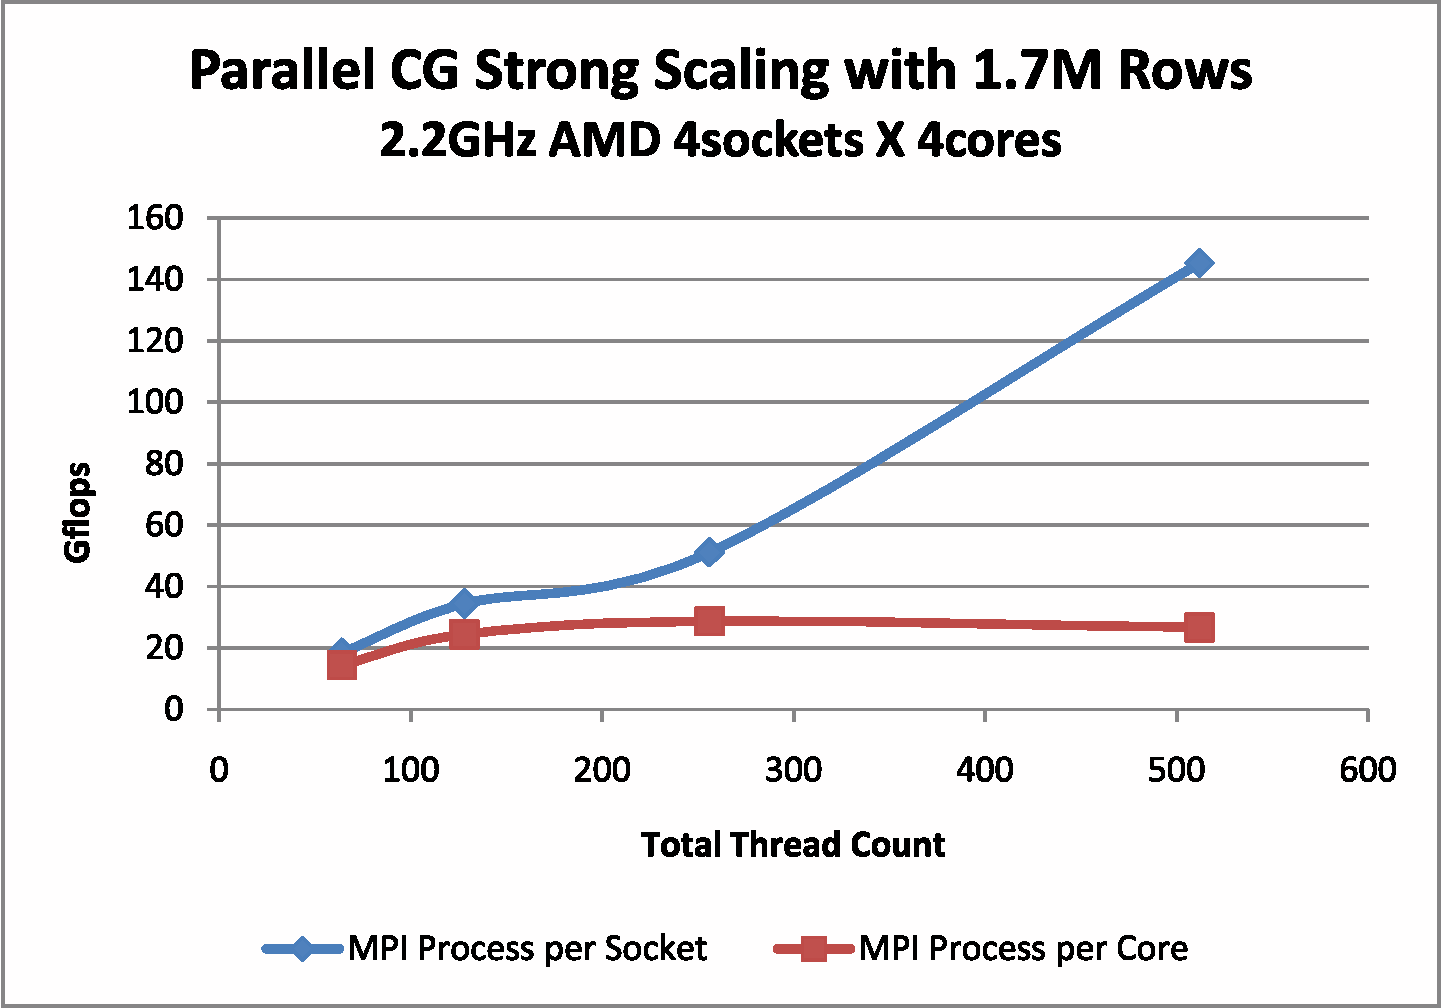
\includegraphics[viewport=1in 0.5in 8.5in 6.5in,angle=0,scale=0.5]{figures/StrongScaling1700k}
\caption{Hybrid parallel conjugate gradient iteration strong scaling for 1.7M rows: one MPI process with 4 threads per CPU socket versus one MPI process per CPU core.}
\label{fig:CGPerf:scaling1.7M}
\end{figure}


\begin{figure}[h]
\center
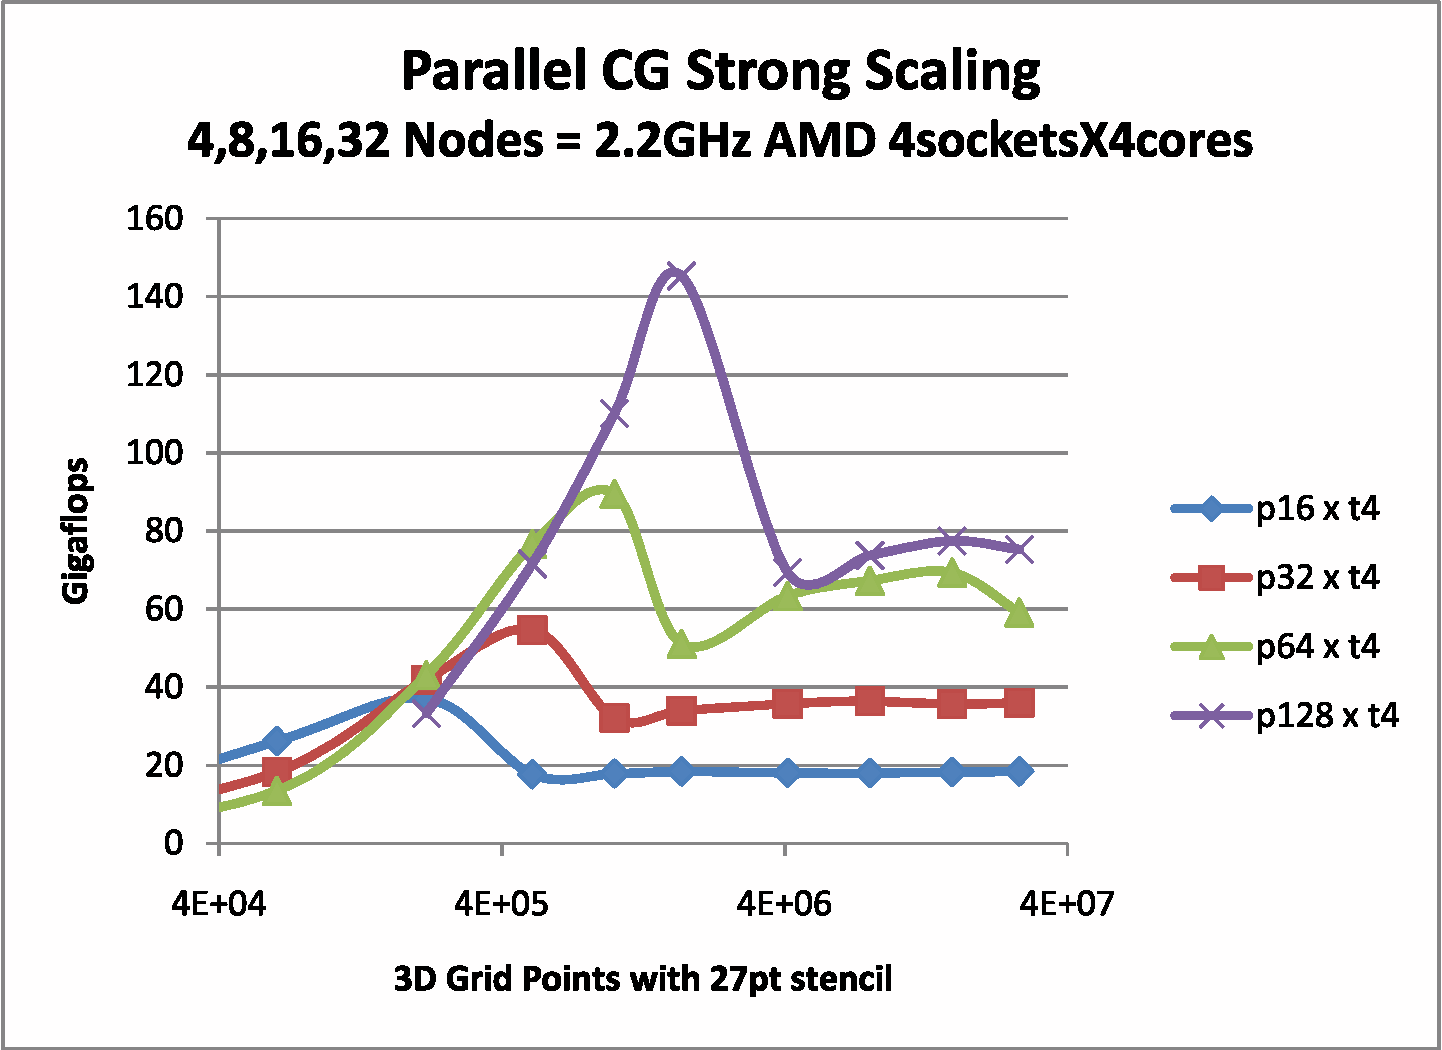
\includegraphics[viewport=1in 0.5in 8.5in 6.5in,angle=0,scale=0.5]{figures/test-hhpccg-intel-11-1-mpi-exe-scaling-no-overlap-2}
\caption{Hybrid parallel conjugate gradient iteration strong scaling with one MPI process and 4 threads per CPU socket.  Strong scaling over 64, 128, 256, and 512 threads is observed for a range of problem sizes by noting the associated problem-size point on each curve.}
\label{fig:CGPerf:scaling}
\end{figure}


\clearpage

\subsubsection{Fused Parallel Kernels}

Thread-parallel performance is most significantly improved by fused parallel kernels,
as per Algorithms~\ref{alg:CG-fused}~and~\ref{alg:FusedMXV},
when thread start/completion overhead is costly compare to kernel's computational costs.
%
This result can be seen in Figures~\ref{fig:CGPerf:np4:fusing}~and~\ref{fig:CGPerf:np32:fusing},
where CG iteration performance improvements are greater for small matrices than for larger matrices.
%
In these graphs the speed up is computed as the performance difference between the fused parallel kernel and conventional parallel kernel implementations, divided by the performance of the conventional parallel kernel implementation.


\begin{figure}[h]
\center
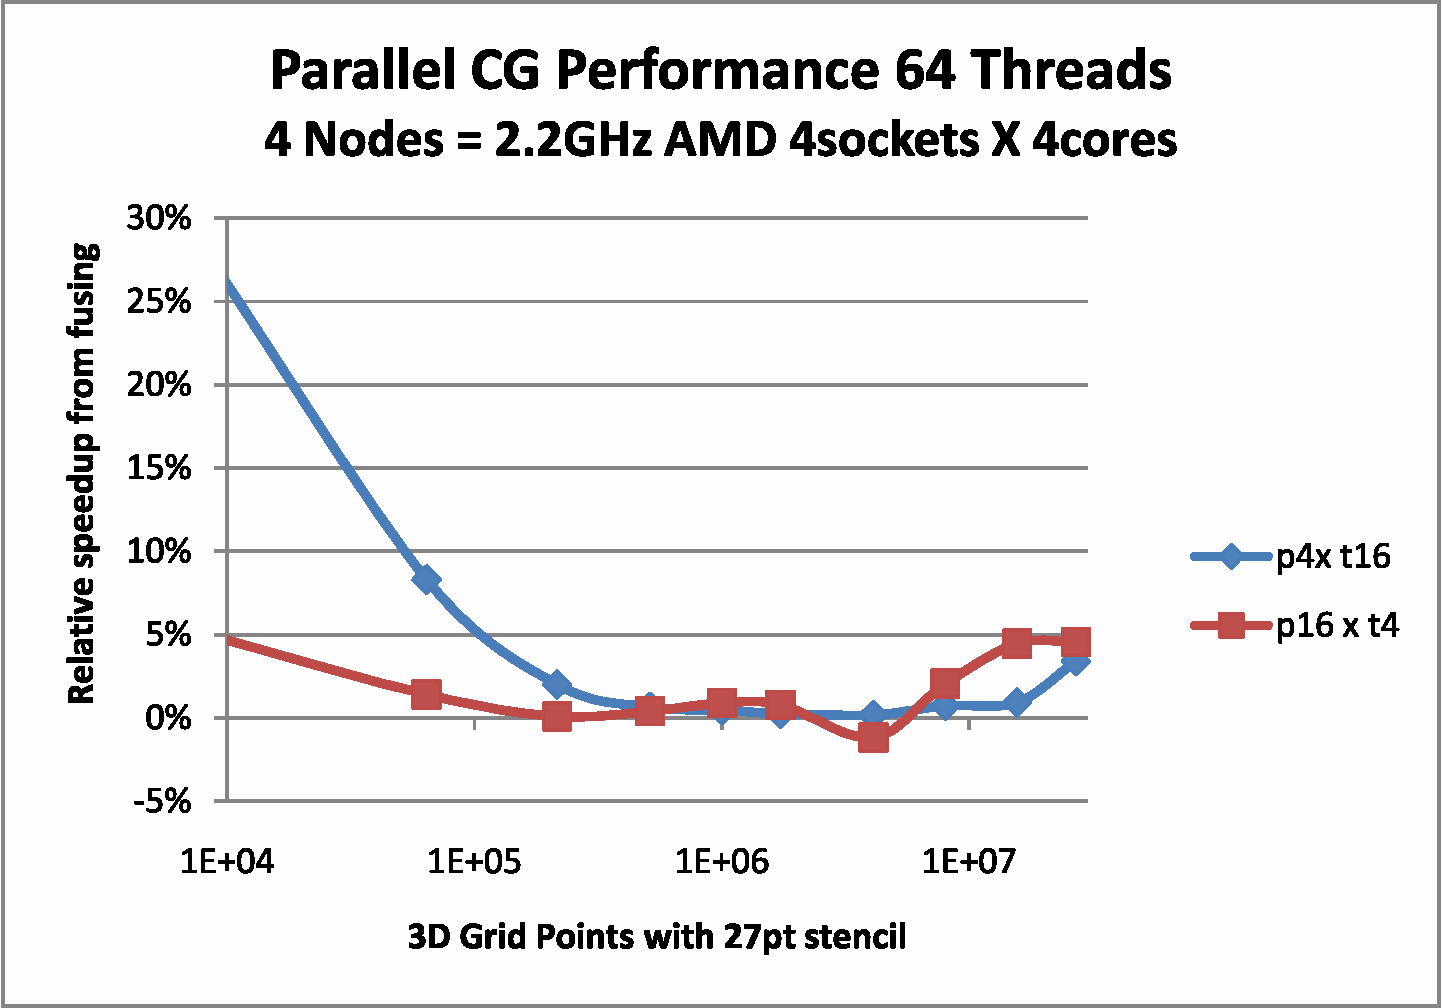
\includegraphics[viewport=1in 0.5in 8.5in 7in,angle=0,scale=0.5]{figures/test-hhpccg-intel-11-1-mpi-exe-np4-no-overlap-fusing}
\caption{Hybrid parallel conjugate gradient iteration relative performance improvement for parallel fused kernels with 4 compute nodes and 64 threads: p4 x t16 = one MPI process per node and p16 x t4 = one MPI process per socket.}
\label{fig:CGPerf:np4:fusing}
\end{figure}

\begin{figure}[h]
\center
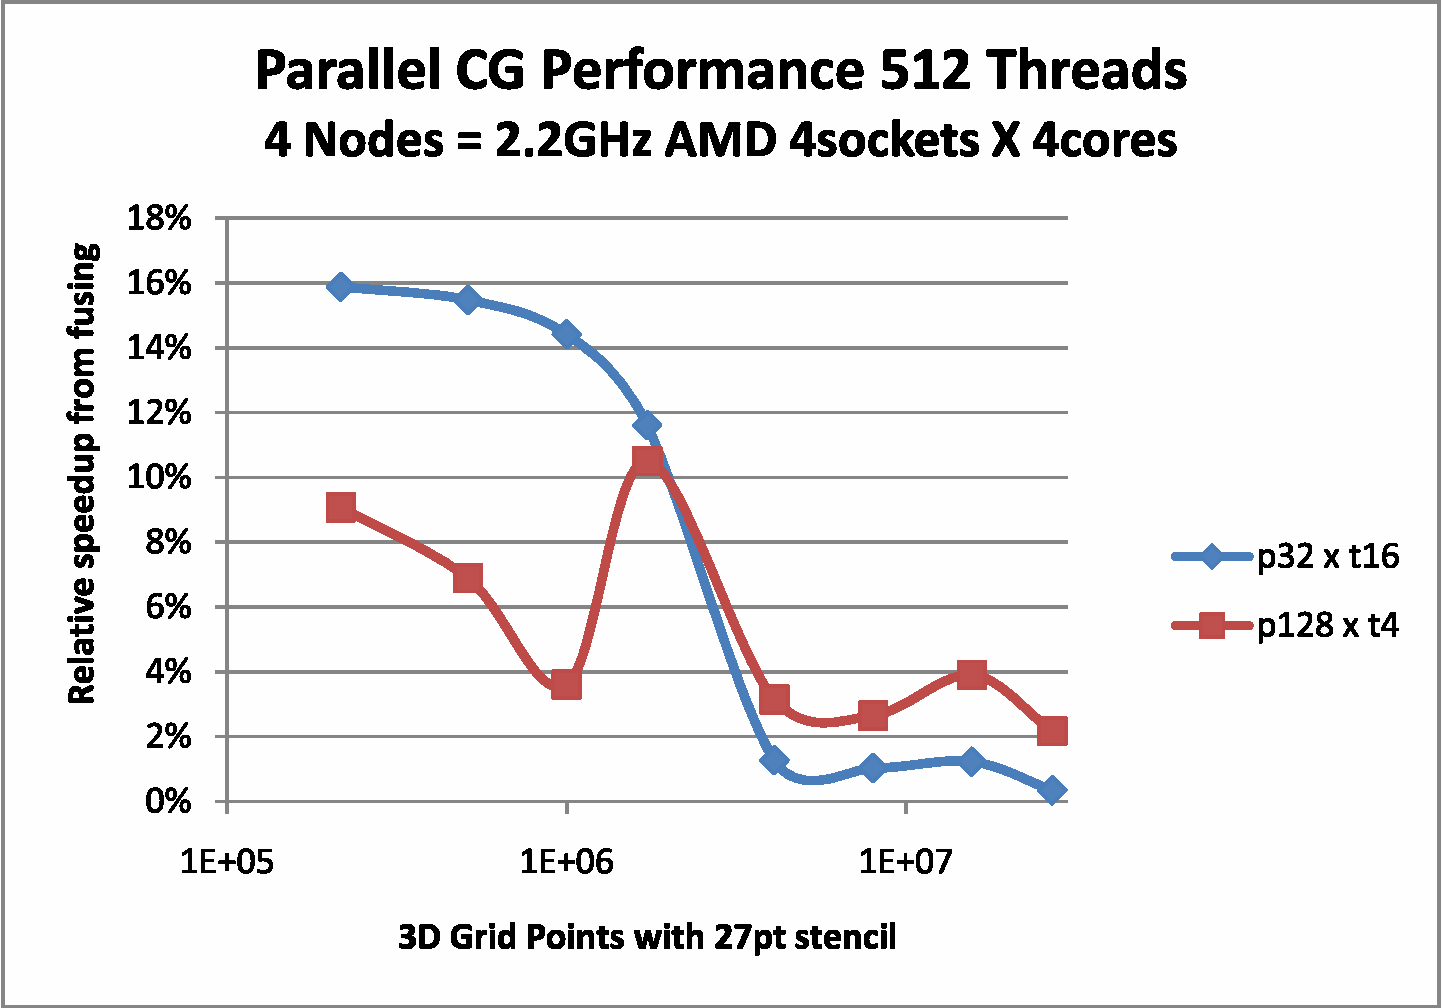
\includegraphics[viewport=1in 0.5in 8.5in 7in,angle=0,scale=0.5]{figures/test-hhpccg-intel-11-1-mpi-exe-np32-no-overlap-fusing}
\caption{Hybrid parallel conjugate gradient iteration relative performance improvement for parallel fused kernels with 32 compute nodes and 512 threads: p32 x t16 = one MPI process per node and p128 x t4 = one MPI process per socket.}
\label{fig:CGPerf:np32:fusing}
\end{figure}
















